\subsection{VisTool}

\begin{figure}
    \centering
    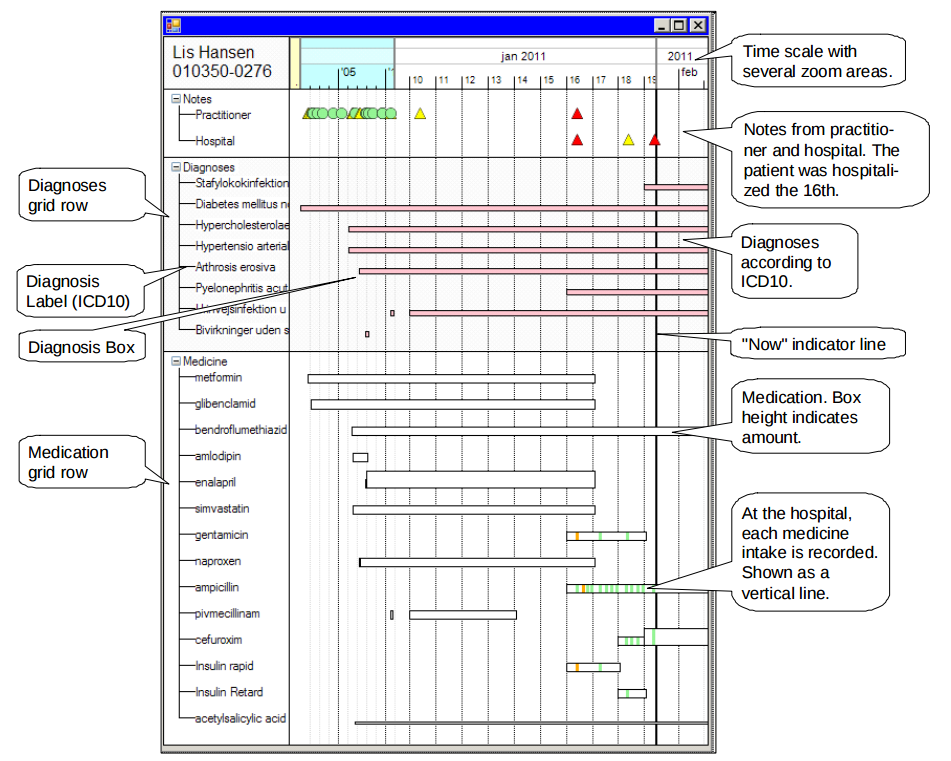
\includegraphics[width=1\textwidth]{images/lifeline.png}
    \caption{A lifeline as being generated by Uvis. Source:~\cite{lauesen2012}.}
    \label{img:lifeline}
\end{figure}

VisTool (Uvis) is a specific type of meta-design model originally created by Søren Lauesen. It emphasis on the construction of user interfaces along with visualization of relation data. It intends to enable users to participate in the design process in collaboration with end-user developers that we will refer to using the term designer. Through a drag-drop-set-property approach, a designer can build and tailor the user interface as unwitting programmer\cite{Costabile2008} --without doing real programming--. Uvis can be used in various contexts but outstands as a solution of it's own kind when it comes to enable non-expert developers to build advanced visualisations such as Lifelines~\cite{Plaisant1998} which shows to be particularly helpful for monitoring data in medical record systems for instance. Figure~\ref{img:lifeline} shows an example of a lifeline as being generated by Uvis.

Other tools exist that allows users to construct screens by dragging and dropping components and to set their respective properties (size, color, position etc.). These make it easy to create ``static'' screens that can work as mock-ups. However, in order to produce screens embedding data which is dynamic and that can vary over time, all of them will require the need of a professional programmer. No tool offers a satisfying tradeoff between the simplicity of use of a drag-and-drop interface and the complexity required to visualize dynamic data.

Charting tools available in spreadsheet systems (Excel, Google spreadsheet etc.), Graphic libraries available for most programming languages, Visualization Toolkits such as D3 for JavaScript, Data analysis tools are examples of other data visualization tools. They all at a certain extent require programming skills and if not, they do not permit to create visualizations beyond what is initially featured by the system.~\cite{lauesen2013}

Uvis provides a design mode --the mode under which the designer can operate the system-- in which a toolbox with an available list of components is available an from where components can be instantiated into the visualization screen by a simple drag-and-drop action from the designer. When most tools typically allow to only assign a static value as a component's property, Uvis allows to express a formula, a simple expression --that reminds of what spreadsheet expressions can look like in tools such as Excel-- that is evaluated into the actual value of the component's property. Through the formula, the designer can address entities from various sources from external data (e.g. resources from the database) to properties from the current or from another component. The actual values of the retrieved entities being addressed are used as the operands in the operations expressed by the designer within a formula. The mechanism through which he addresses things is very central and is referred to as the \emph{walk principle}~\cite{lauesen2013}. The formula gives the sufficient expressive power for the designer to express rules which can be used to generate complex interfaces such as the lifeline, with no or very little amount of programming knowledge. I talk more in detail about formulas, the walk principle and the context in which formulas can be declared in the language description in section~\ref{sec:languageDescription}.

The current system is developed in C\# as a visual studio solution and is designed to run locally on a computer. It's entire architecture builds around the assumption that any resource, other that the external data, can be found and accessed locally. With the emergence of the web, many users are expecting to see their software products as a web based client running in their favorite Browser. Uvis offers unique capabilities in terms of data-visualization and by showing the feasibility of bringing such capabilities into the browser I hope to participate in the debate about meta-design models for data-visualization. \todo[inline]{I would appreciate some help to reformulate this last sentence.}